\documentclass[11pt,a4paper]{article}
\usepackage[T1]{fontenc}
\usepackage[margin=23mm]{geometry}
\usepackage{graphicx}
\usepackage{booktabs}
\usepackage{amsmath}
\usepackage{xcolor}
\usepackage[hidelinks]{hyperref}
\definecolor{reportblue}{RGB}{26,64,87}
\setlength{\parindent}{0pt}
\setlength{\parskip}{6pt}
\renewcommand{\arraystretch}{1.15}
\newcommand{\filepath}[1]{\nolinkurl{#1}}
\newcommand{\pagetitle}[1]{\section*{#1}}

\begin{document}
\begin{center}
{\Large\bfseries\color{reportblue} Machine Failure Classification}\\[5pt]
{\large Dataset, Splitting Approach, and Baseline Results}\\[6pt]
\textbf{maintain-predict}\quad |\quad 17 November 2026
\end{center}

\textbf{Scope.} This report records completed work: dataset inspection and
exploratory analysis, the agreed target definition, the manually executed data
split, and the executed scikit-learn baseline experiment. All model results
are from the validation partition. No new training was performed to produce
this report, and the final test partition has not been evaluated.

\pagetitle{1. Dataset overview}
The uploaded AI4I 2020 file is a synthetic predictive-maintenance dataset with
\textbf{10,000 observations and 14 columns}. Each row contains operating
measurements, a product category, identifiers, and recorded failure outcomes.
A row is an observation, not a complete machine maintenance history.

The model uses \textbf{six inputs}: one categorical feature and five numeric
measurements. Identifiers and outcome annotations are excluded from inputs.

\begin{center}
\begin{tabular}{llr}
\toprule
Input & Unit or categories & Observed range \\
\midrule
Type & L, M, H & 3 categories \\
Air temperature & K & 295.3--304.5 \\
Process temperature & K & 305.7--313.8 \\
Rotational speed & rpm & 1,168--2,886 \\
Torque & Nm & 3.8--76.6 \\
Tool wear & min & 0--253 \\
\bottomrule
\end{tabular}
\end{center}

Type counts are L: 6,000; M: 2,997; and H: 1,003. Tool wear represents
accumulated usage. The outcome columns are \texttt{Machine failure} and the
five mode flags: TWF (tool wear), HDF (heat dissipation), PWF (power), OSF
(overstrain), and RNF (random failure).

\textbf{Quality checks.} The file has no missing cells, no duplicate complete
rows, and no duplicate combinations of the six model inputs. Type values are
valid, and the recorded outcome columns contain binary values. The raw CSV
has been preserved unchanged. Unusual sensor values were retained rather
than removed solely because an outlier rule identified them.

\textbf{Prediction scope.} There are no timestamps, explicit forecast horizons,
or remaining-useful-life labels. The current task is classification of recorded
failure evidence; these results do not establish prediction of a future failure
within a specified time window.

\newpage
\pagetitle{2. Target policy and exploratory findings}
\subsection*{2.1 Recorded-label disagreements}
The original \texttt{Machine failure} label contains 339 positives (3.39\%).
Comparing it with the presence of any failure-mode flag reveals 27 disagreements:

\begin{center}
\begin{tabular}{ccrr}
\toprule
Original failure & Any mode flag & Rows & Derived target \\
\midrule
0 & 0 & 9,643 & 0 \\
0 & 1 & 18 & 1 \\
1 & 0 & 9 & 1 \\
1 & 1 & 330 & 1 \\
\bottomrule
\end{tabular}
\end{center}

All 18 original negatives with a positive flag are RNF-positive. The nine
original positives without any mode flag were also retained as positives.

\subsection*{2.2 Agreed modeling target}
The project defines a separate target, \texttt{Failure evidence}, under policy
\filepath{failure_evidence_or_v1}:
\[
y = \text{Machine failure} \lor \text{TWF} \lor \text{HDF}
    \lor \text{PWF} \lor \text{OSF} \lor \text{RNF}.
\]
This rule produces \textbf{357 positives (3.57\%)} and 9,643 negatives. It
promotes 18 original negatives, demotes no original positives, and retains
all 10,000 observations.

The rule is a documented \textbf{positive-evidence assumption}. It does not
verify which source annotation is correct. The increased positive fraction
is a consequence of the policy, rather than evidence of improved label
quality. RNF-positive examples may lack a predictable sensor pattern.

Outcome flags, the original overall label, and the derived target are used
for label construction or auditing only. Including them in the input matrix
would reveal target information and create leakage. UDI and Product ID are
also excluded from model inputs.

\subsection*{2.3 Completed exploratory analysis}
The executed EDA notebook examined schema, missing values, duplicates,
sensor summaries and distributions, Type, class balance, correlations,
scatter plots, label disagreements, and original row order.

The class is strongly imbalanced. Air and process temperatures are positively
correlated (approximately 0.876), while speed and torque are negatively
correlated (approximately $-0.875$). Tool-wear averages are similar across
Types, so an additional below/above-average wear grouping was not adopted.

Adjacent rows have strongly correlated temperatures. Therefore, a random
split measures performance on this allocation and does not demonstrate
generalization to a later operating period. Whole-file EDA was performed
before splitting; the test partition is reserved from model evaluation,
but was not completely unseen during descriptive analysis.

The notebook uses the derived target. Earlier dashboard and descriptive-report
views remain explicitly marked as original-label reference snapshots.

\newpage
\pagetitle{3. Splitting approach}
The agreed allocation is \textbf{70\% training, 15\% validation, and 15\% test},
with random seed \textbf{42}. Stratification uses the joint category
\(\text{Type} \times \text{Failure evidence}\), giving six strata.

The manual exercise performs two splits: first 70\% training and 30\% held
out, then an equal split of that held-out portion into validation and test.
Both stages preserve the joint strata as closely as whole-row allocation allows.
Tool wear remains a numeric predictor, rather than a splitting group.

\begin{center}
\begin{tabular}{lrrrr}
\toprule
Partition & Rows & Positive & Negative & Positive rate \\
\midrule
Training & 7,000 & 250 & 6,750 & 3.571\% \\
Validation & 1,500 & 54 & 1,446 & 3.600\% \\
Test & 1,500 & 53 & 1,447 & 3.533\% \\
\bottomrule
\end{tabular}
\end{center}

\begin{center}
\begin{tabular}{ccrrr}
\toprule
Type & Target & Training & Validation & Test \\
\midrule
L & 0 & 4,027 & 863 & 863 \\
L & 1 & 173 & 37 & 37 \\
M & 0 & 2,038 & 437 & 437 \\
M & 1 & 60 & 13 & 12 \\
H & 0 & 685 & 146 & 147 \\
H & 1 & 17 & 4 & 4 \\
\bottomrule
\end{tabular}
\end{center}

\textbf{Balance diagnostic.} Mean tool wear is 107.584 minutes in training,
108.994 in validation, and 108.621 in test. These similar means are allocation
diagnostics, not performance measurements. Only four H-positive observations
are present in each held-out partition, limiting subgroup conclusions.

\textbf{Frozen allocation.} The user ran
\filepath{scripts/01_split_data.py}. The resulting manifest,
\filepath{data/splits/type_target_seed42.json}, stores source-row membership,
UDI values, source checksum, target policy, seed, and split settings. Model
runs load this existing allocation rather than generating another split.

\textbf{Verification.} The saved partitions are pairwise disjoint, cover every
source row exactly once, have the agreed sizes, and match the source UDI
values and SHA-256 checksum. Positive counts and validation prediction-row
membership were checked again while preparing this report.

\textbf{Partition roles.} Training fits preprocessing and model parameters.
Validation measures baseline performance. The test partition remains reserved
for final model evaluation; the class counts above describe allocation only.

\newpage
\pagetitle{4. Baseline experiment and validation metrics}
The user executed \filepath{scripts/02_baselines.py}. Both approaches use
the same frozen split and are evaluated on the same 1,500 validation rows.
No PyTorch training was performed.

\subsection*{4.1 Always-no-failure reference}
\texttt{DummyClassifier(strategy="constant", constant=0)} always predicts
no failure evidence. Its \texttt{fit} call establishes sklearn class metadata;
it does not learn relationships between inputs and the target. It is a
reference rule showing what high accuracy can mean on an imbalanced dataset.

\subsection*{4.2 Balanced logistic regression}
The scikit-learn pipeline combines one-hot encoding of Type, standardization
of the five numeric sensors, and logistic regression. Encoding and scaling
are fitted on training rows only. Validation uses those fitted transformations.
With all three Types present, the transformed input contains eight columns.

For each sensor, standardization applies
\(z=(x-\mu_{\mathrm{train}})/\sigma_{\mathrm{train}}\).

The classifier uses
\texttt{class\_weight="balanced"}, \texttt{solver="lbfgs"},
\texttt{max\_iter=2000}, and seed 42. Balanced weighting changes the loss
contribution of existing rows; it does not add failure observations.
The training counts imply class weights of approximately 0.519 for negatives
and 14.0 for positives.

\begin{verbatim}
logistic = make_logistic_pipeline(random_state=42)
logistic.fit(X_train, y_train)
scores = logistic.predict_proba(X_validation)[:, 1]
predictions = (scores >= 0.5).astype(int)
\end{verbatim}

The threshold is fixed at \textbf{0.5}, not tuned. Weight updates use training
data; validation labels are used for evaluation, not gradient updates.

\subsection*{4.3 Saved validation results}
\begin{center}
\begin{tabular}{lrr}
\toprule
Metric & Always no failure & Logistic regression \\
\midrule
Accuracy & 96.40\% & 80.07\% \\
Precision & Undefined & 13.65\% \\
Recall & 0.00\% & 85.19\% \\
F1 & 0.00\% & 23.53\% \\
Average precision (AP) & 0.0360 & 0.5288 \\
Predicted positives & 0 & 337 \\
\bottomrule
\end{tabular}
\end{center}

Precision is undefined for the dummy because it raises no alarms. Its F1 is
reported as zero by the evaluation convention. AP summarizes score ranking
across thresholds; it is not precision at 0.5 or trapezoidal PR area. Constant
dummy scores give AP equal to validation prevalence, \(54/1500=0.036\).

\newpage
\pagetitle{5. Confusion matrices and interpretation}
The positive class means \emph{failure evidence is present}; ``positive'' does
not mean good. A true positive detects a positive label, a false negative
misses one, and a false positive is an alarm on a negative label.

\begin{center}
\begin{tabular}{llrr}
\toprule
Prediction & Actual label & Always no failure & Logistic \\
\midrule
No evidence & No evidence (TN) & 1,446 & 1,155 \\
No evidence & Evidence (FN) & 54 & 8 \\
Evidence & No evidence (FP) & 0 & 291 \\
Evidence & Evidence (TP) & 0 & 46 \\
\bottomrule
\end{tabular}
\end{center}

\begin{center}
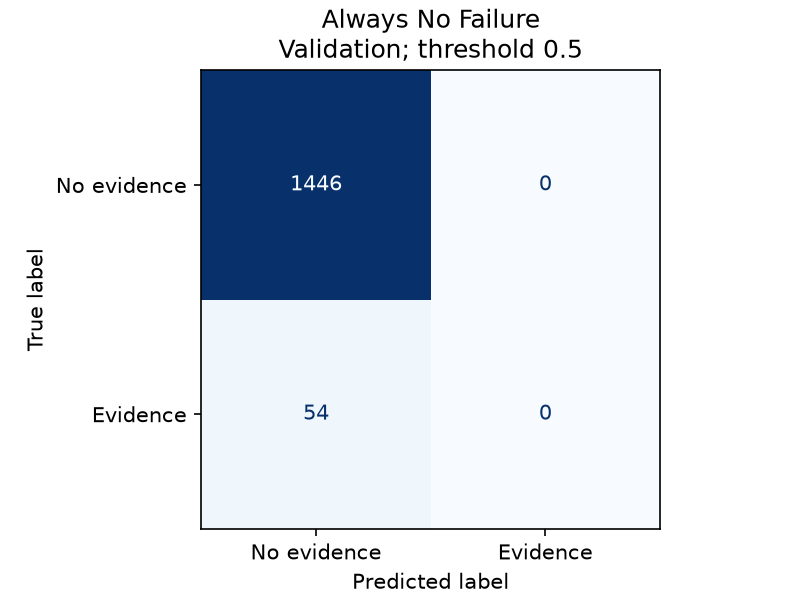
\includegraphics[width=0.48\linewidth]{figures/always_no_failure_confusion_matrix.png}
\hfill
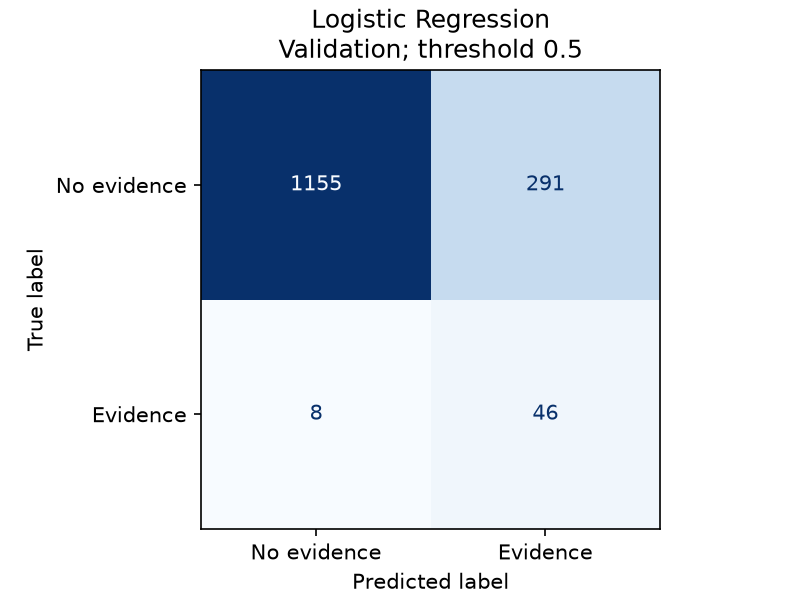
\includegraphics[width=0.48\linewidth]{figures/logistic_regression_confusion_matrix.png}

{\small Saved validation plots. Rows are actual labels; columns are predictions.}
\end{center}

The dummy correctly identifies every negative observation but misses all
54 positives. Logistic regression detects \textbf{46 of 54 positives} and
misses 8, while generating \textbf{291 false alarms}. It raises 337 alarms
in total, of which only 46 agree with positive actual labels.

\[
\begin{aligned}
\text{Accuracy} &= \frac{TP+TN}{TP+TN+FP+FN}
                = \frac{46+1155}{1500} = 80.07\%,\\
\text{Recall} &= \frac{TP}{TP+FN}
              = \frac{46}{54} = 85.19\%,\\
\text{Precision} &= \frac{TP}{TP+FP}
                 = \frac{46}{337} = 13.65\%.
\end{aligned}
\]

The learned baseline reduces missed positives from 54 to 8, at the cost of
291 additional false alarms. Its lower accuracy does not contradict its
higher recall: the two metrics count different aspects of performance.
No operational cost assumptions have been established, so this tradeoff
does not establish readiness for deployment.

These counts are disagreements or agreements with the \emph{derived dataset
labels}, not independently verified physical machine outcomes. Class-weighted
scores should not automatically be interpreted as calibrated real-world risks.

\newpage
\pagetitle{6. Reproducibility, artifacts, and completion boundary}
\subsection*{6.1 Recorded environment and experiment identifiers}
The saved experiment summary records Python 3.14.3, NumPy 2.5.4,
pandas 3.1.1, scikit-learn 1.9.1, MLflow 3.18.0, and skops 0.16.0.
Local MLflow tracking stores run metadata and artifacts. The saved run IDs are:

\begin{tabular}{ll}
Always no failure & \texttt{7d06668798524b0585917072719d8841} \\
Logistic regression & \texttt{457b45c83e8b428b817082227d733b1b} \\
\end{tabular}

The unchanged source file, \filepath{data/ai4i2020.csv}, has SHA-256:
\begin{verbatim}
dc6630cd9b1f0f853922fad78a1b6436570d3f1ec863f1dd5c4340ac56bc8a8e
\end{verbatim}

\subsection*{6.2 Evidence files}
All paths below are relative to the project root.
\begin{itemize}
\item \filepath{notebooks/01_eda.ipynb}: executed exploratory analysis.
\item \filepath{docs/target_policy.md}: agreed label definition and limitations.
\item \filepath{docs/split_verification.md}: allocation checks and stratum counts.
\item \filepath{data/splits/type_target_seed42.json}: frozen row membership.
\item \filepath{src/maintain_predict/train.py}: unfitted pipeline factory.
\item \filepath{scripts/02_baselines.py}: manually executed training exercise.
\item \filepath{artifacts/baselines/results.json}: metrics, environment, run IDs,
target policy, source checksum, and explicit \texttt{test\_evaluated=false}.
\item \filepath{artifacts/baselines/comparison.csv}: comparison of validation metrics.
\end{itemize}

Each baseline subfolder also contains \filepath{model.skops},
\filepath{validation_predictions.csv}, \filepath{validation_metrics.json},
and saved confusion-matrix and precision--recall plots.

Report verification checked the raw-file checksum against both the manifest
and experiment summary, recalculated the partition positive counts, and
reconstructed both confusion matrices from saved predictions. No models were
refitted, no split was regenerated, and no test predictions were generated.

\subsection*{6.3 What is and is not complete}
Dataset inspection, EDA, target-policy documentation, stratified splitting,
the dummy baseline, balanced logistic-regression training, validation
evaluation, and local experiment tracking are complete.

This report makes no claims about completed cross-validation, random-forest
or XGBoost comparisons, engineered-feature experiments, threshold optimization,
probability calibration, row-block sensitivity analysis, SHAP explanations,
final test performance, model registration, or deployment. These activities
have not been performed in the reported baseline experiment.

The current evidence is limited to a synthetic dataset, an assumed label
policy, and one stratified random allocation. Strong row-order dependence,
rare positive examples, prior whole-file EDA, and a substantial false-alarm
count limit broader conclusions.

\end{document}
